\subsection{Hardware Details}
\subsubsection{Deployment device}

\begin{description}
%organ pipe already introduced?
%pig? calibration device, source deployment mechanism.
\item The calibration device (the so called "pig") is deployed in the \lsv and thereby gets immersed in the liquid scintillator. The liquid scintillator however may not get in touch with oxygen or water, and therefore the apparatus is completely sealed during deployments to maintain the liquid scintillator under a nitrogen blanket 100\% of the time.
%tested for helium leak tightness

\item The source may not get in contact with the liquid scintillator. It is therefore sealed during the deployment in a dedicated source holder. In order to exchange sources the source arm and source holder has to be extracted from the pig into CRH and thereby comes in contact with normal air, containing oxygen and traces of water. After insertion a flush \& purge cycle is used to reduce, as known from glove boxes. No glove box present. Much more compact design.
% no glove box

\end{description}


\subsubsection{Deployment device (``pig'')}

The overall device consists of three main assemblies: the lower assembly, upper assembly, and the source deployment mechanism. Fig \ref{fig:wholeAssembly_insideDetectors} shows the layout of the system as installed CRH and deployed in Liquid Scintillator Veto (LSV). Fig. \ref{fig:CALISDimensions3} shows the details of the full device with all dimensions included. The lower assembly (Section \ref{The Lower Assembly}) is attached to the top of the gate valve (that closes the organ pipe in CRH), visible at the bottom of the Fig.\ref{fig:CALISDimensions3} and portruding to the left. On the top of the lower  assembly is a view port  (depicted in blue) and an access point for accessing the arm and exchanging sources. The structure shaped like two joint cones below the viewport guides the system smoothly down the organ pipe. Source capsule is visible inside the blue viewport. Circular gear above the viewport allows the rotation of the source arm to horizontal position as shown. The second conical cap above the rotation gear mechanism contains a cylindrical weight to minimize any lateral motion or oscillations during deployment and articulation and dearticulation especially. It also ensures smooth motion of the CALIS III into the organ pipe and back to the top park position. Fig \ref{fig:sourcePod_arrows} shows the photo of these parts as assembled. Inside the upper assembly (Section \ref{The Upper Assembly}) that attaches to the lower assembly are the two spools (shown in profile) used to wind and unwind two cables that hold the deployment mechanism simultaneously. The spools are attached to a single shaft rotated by the stepper motor drive shown at the top right side of the upper assembly. Small circular object located at the top left of the upper assembly is the manual handle for source arm articulation to horizontal position and back to vertical position during deployments.  The drive mechanism is controlled via a LabVIEW interface (Section \ref{LabView}).  The third assembly of the device that contains the source deployment mechanism is called "the pig", Section \ref{The Pig}. It encompases the arm, the source container (located at the end of the arm), and two conical shells (mentioned above) for the smooth transportation of the source  (again see Fig \ref{fig:sourcePod_arrows} for details). The pig is stored in the upper assembly, with the source arm in view, through the view port of the lower assembly. This allows the gate valve to remain closed except during calibration of the detector. During deployments the whole pig is lowered into the detector. 

\begin{figure}[htbp]
 \centering
  \includegraphics[width= 8.5in]{Figs/sourcePod_arrows}
  \caption{The pig-support for the arm and the source holder.}
  \label{fig:sourcePod_arrows}
\end{figure}

 \subsection{The Lower Assembly} \label{The Lower Assembly}
 \paragraph{}
    The lower assembly is a cylindrical stainless steel enclosure pipe that contains the ports for viewing and accessing the source and the cables on its upper end. The front view/access port can be opened for easy manipulation/handling of the source. Below the view port is a sealed connection that has an o-ring seal and uses a ring clamp to compress the seal. The clamp can be slightly loosened to allow the entire upper assembly with the pig to be rotated with respect to the lower assembly and the detector. Refer to Fig. \ref{fig:Rotation2} for a conceptual description of the device rotation with respect to the detector and the assemblies). The angle rotation is read out from the measuring strip. The ring clamp and the measuring strip are shown in Fig.~\ref{fig:ring_clamp}. During the rotation in the xy-plane, light and air tightness are preserved. Thus, the rotation of the pig can be performed, while the pig is deployed next to the cryostat (and open  gate valve).  The lower assembly is connected to the gate valve on top of the organ pipe in CRH.  The distance from the center of the viewing port to the top of the gate valve flange is 74.85\,cm (29.47\,inches). This distance was based on a person sitting comfortably in a chair while handling the source.  Fig. \ref{fig:lowerAssembly_dimensions} shows the dimensions of the lower assembly and the upper and lower assemblies connected as they will be in CRH in comparison to a person of average height.   When the source arm is centered in the view port, the view port may be opened for handling of the source.  This is considered the home position for the pig.  

\begin{figure}[htbp]
 \centering
  \includegraphics[scale=0.5]{Figs/RingClamp.jpg}
  \caption{Ring clamp  with the angle measuring strip shown below. In order to perform azimuthal rotation, ring clamp is slightly loosened, and the entire upper assemby is rotatated with respect to the lower assembly, along with the pig. The angle of rotation is read out from the strip that goes around the pipe. }
  \label{fig:ring_clamp}
\end{figure} 

	
 \subsection{The Upper Assembly} \label{The Upper Assembly}
The upper assembly is a stainless steel cylindrical enclosure that houses the drive mechanism and the gear drive for the cables. The raising and lowering of the source is controlled by a servo motor drive which is operated via a LabVIEW interface (Sec. \ref{LabView}).  The motor controls z positioning of the source by simultaneously unwinding and winding a pair of cables  that the pig is attached to.  We are able to specify in LabVIEW a z position that we want the source to be in and command it to go there.  In order to move up or down in z motor is given a certain number of steps to go. There is a translation table that gives correspondence between each z positiona and number of steps on the motor. The motor has an absolute encoder and step position is never lost even in the case when the motor loses power. When the pig has reached its home position within the upper assembly it will stop.  However, if the top of the pig continues past its home position (based on the number of steps given), it will not be able to pass its home position thanks to the upper limit switch that will be triggered in that case. When contact is made with the switch, it will trip the upper limit and open the circuit, turning off the 24 Volts line powering the motor.  This would be considered a system failure and the problem will need to be understood and corrected before continuing.   
 Fig.~\ref{fig:limit_switch} shows the schematic of the connection between the limit switch and the motor.

	
 \subsection{The Pig} \label{The Pig}
The pig (Fig. \ref{fig:sourcePod_arrows}) contains the support structure for the arm which holds the source at its end.  This piece is equipped with tapered cones on the top and bottom that ensure that the ends do not get snagged on inner edges of the organ pipe as it is moving up and down. It is attached to the assembly by the two cables.  Swivel hooks are employed in the attachment of the cables to the pig that allow the cables to move freely and not get tangled.  There is a chain that goes from the swivel hook around the gear to the second swivel hook. In the center of the gear is a custom designed and fabricated source arm pivot that the arm is attached to and that rotates together with the articulation gear visible in the center of the pig. See Fig. \ref{fig:SourcePod2} for an image of the arm raised to its horizontal position.  
 
\subsection{Source arms}
  For articulation, there is currently a choice of three arm lengths---40.31\,cm,  57.15\,cm and 62\,cm.  Each of these lengths are measured from the center line of the organ pipe to the end of the source holder.  The arm lengths, 57.15\,cm and 62\,cm are intentionally made too long as they will be used to determine the exact location of the cryostat; some uncertainty in the cryostat's z and lateral position exist at the level of 3 - 4\,cm. The organ pipe we intend to use is 81\,cm distant from the cryostat center (and the geometric center of the LSV sphere) as measured from the center line of the organ pipe. The cryostat is 32\,cm in radius, which leaves a distance of $\sim$49\,cm to be reached  by the arm.  The articulation of the arm is operated via a hand wheel located on the side of the upper assembly close to the top.  By rotating the hand wheel, one of the cable spools inside the upper assembly will rotate which pulls up on one of the cables attached to the pig and shortens it for the length equal to the one quarter of the gear curcamference (which is 10\,cm).  As a result, the chain at the bottom of the cables engages the articulation gear (see Fig. \ref{fig:sourcePod_arrows} for an image of the articulation gear) on the pig and raises the arm to horizontal.  The chain has a guard rail that ensures that chain can never come of the gear. Thus, in the process of articulation the entire pig along with the source arm shifts up for 10\,cm.  See Fig. \ref{fig:pigAndCables_fullView} and  Fig. \ref{fig:sourceArmRotation} for a closer look at how CALIS III articulates the arm. In order to determine the degree of articulation of the arm, a protractor is placed next to the hand wheel.  This protractor and the hand wheel are calibrated together for an accurate reading of the articulation. The reading of the protractor dial is different at different heights and calibration table obtained from the tests is used to determine the dial setting necessary to articulate the arm to horizontal position. We have adopted a spherical coordinate system for the rotation of the system and the articulation.  Articulation of the arm is measured in $\theta$ from the z-axis; when the arm is fully articulated, it is at 90$^{\circ}$ and when it is in its vertical position it is at 180$^{\circ}$.  As mentioned in Sec. \ref{The Lower Assembly}, the rotation of CALIS III is done in the xy-plane which corresponds to the azimuthal direction, a rotation in $\phi$.  See Fig. \ref{fig:coordinate_system} for details. 
  
\begin{figure}[htbp]
 \centering
  \includegraphics[width=7in]{Figs/pigAndCables_fullView.png}
  \caption{CALIS III showing the inner workings of the articulation of the arm and the arm in its vertical position. }
  \label{fig:pigAndCables_fullView}
\end{figure}


\subsection{Degrees of freedom of the system}
\begin{figure}[htbp]
 \centering
  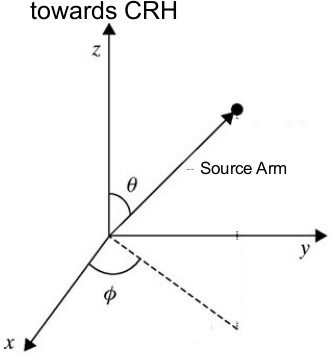
\includegraphics[scale=0.9]{Figs/coordinate_system}
  \caption{Spherical coordinate system used for establishing the direction of the rotation of CALIS-III and the articulation of the source arm. $\theta$ is kept at 90$^{\circ}$ when arm is articulated, and at 180$^{\circ}$ when dearticulated. $x$-axis is the direction toward the center of the detector. }
  \label{fig:coordinate_system}
\end{figure} 
	
 \subsection{Safety features} \label{Safety Features}
  \paragraph{} 
 CALIS III offers various safety features to ensure that the device runs smoothly, no components (especially sources) are lost inside the detector, avoid any contamination of the detector by dirty or incompatible materials, maintain pressure and avoid introduction of oxygen or water in contact with the LS and TMB, operation in the volume that excludes possibility of contact with PMTs or light pulsers (pacman) attached to each PMT.
 
 \begin{itemize}
  \item{Drive Mechanism}
 
   The drive mechanism is a stepper motor that has an integrated absolute encoder providing the location of the source at all times, even in the event of a power failure. The torque of the servo motor is limited in case of an unexpected load.

 \item{Magnectic Break}
 
  In the event of a power failure, the magnetic break ensures there is no movement of the pig. 
  
  \item{Speed Reducer}
  
  The speed reducer (gears) is a double worm gear design. The primary worm gear has a 50:1 reduction and the secondary worm has a 82:1 reduction. The input speed of the servo motor is 2400 RPMs and the output is 0.6 RPM and has the weight capacity of 148 lbs. In the event of a power failure the speed reducer has the ability to hold the load at any position without back drive. The speed of the motor has been limited to 0.4\,cm/s which minimizes any lateral oscillation of the pig during lowering and raising the source. Additionally, this is the maximum speed at which the motor is not overheating.
	
\item{Manual retraction system}

In case of complete motor failure while the source is deployed, it is possible to manually retract the pig back to its home position and close the gate valve. The motor is disengaged, and wrench is used to manually wind the cable back onthe spools and retract the pig back above the gate valve.

\item{Cable strength and cable termination}

The cables holding the pig have been rated for loads over 590\,kg, while the weight of the pig is at the level of 10-15\,kg so well below the breaking strength of the cable. The cable terminations have been crimped with stainless steel crimps and swivel hooks conneted to the thimble of the cable termination.

\item{Cable length}
The cable length has been established so that the maximum depth at which the pig can be deployed is above the level of the PMTs. In case, the command is given to deploy to greater depth, the cable completely unwinds and then rewinds in the opposite direction, which then effectively retracts the pig to a higher z-position until the preset motor count of steps is reached. 

%% is this true?

\item{verticality of the organ pipes}
electrical contact was made, but still quite straight. Dimensions of the organ pipes? Also interesting to report above...


   
\item{Upper limit switch}

There is a limit switch inside the upper assembly that will cut the power to the motor if the pig starts to move above its designated home position.

\item{Articulation retraction limit switch}

Arm retraction limit switch cuts the power to the motor as soon as the arm is not vertical. In this way, any possibility of retracting the arm into the organ pipe while articulated has been eliminated.

\item{Choice of materials}

All materials that come into contact with LS and TMB or their vapors, have been made out of stainless steel, teflon and viton that have been certified as safe in contact with the LS and TMB.


\item{Light covers on the view ports}

All viewports have  very tightly fitting covers. Additionally, the main viewport cover will additionally be held in place with clamps to avoid any possibility of accidently exposing the LSV to excessive amount of light. 
     
\item{Leak tightness of the source holder}

 The source is placed inside a stainless steel container that has an o-ring seal (made out of viton) during calibration. The container has been tested at Fermilab to be helium leak tight.  

\item{tapered cones}
Tapered cones at the top and bottom end of the big minimize the risk of the pig getting tangled while moving up or down. This is a safety precaution, since the organ pipes are free of cables or sensors and 





\item{Securing of the source}

All connection points for the source and arm have been secured with two push locking pins that cannot be disengaged without person pressing the pin. 
The source holder is held in place via a locking mechanism and two locking pins (see Fig \ref{fig:sourceHolder_locking} and Fig. \ref{fig:sourceAttachmentParts}).  When the source is attached to the arm, the source container must be slid over a protruding pin. There is a sliding locking mechanism that interlocks onto the pin. Once the source is locked into position there are 2 additional locking pins that are put into place (one above and one below the source holder pin), each of which have a button that must be depressed in order for the pins to be released.  See DocDB \#858 for two movies in which this mechanism is demonstrated. In addition, the source holder and the 2 locking pins will all be tethered from outside the view port until they are locked in place eliminating the possibility of accidental falling.  The tethering will happen before installation of the source and before the removal of the source. The cables used to tether the pins and the source holder during installation and removal will be detached after installation and prior to deployment to avoid the possibility of the arm getting entangled.  
 
\begin{figure}[htbp]
 \centering
 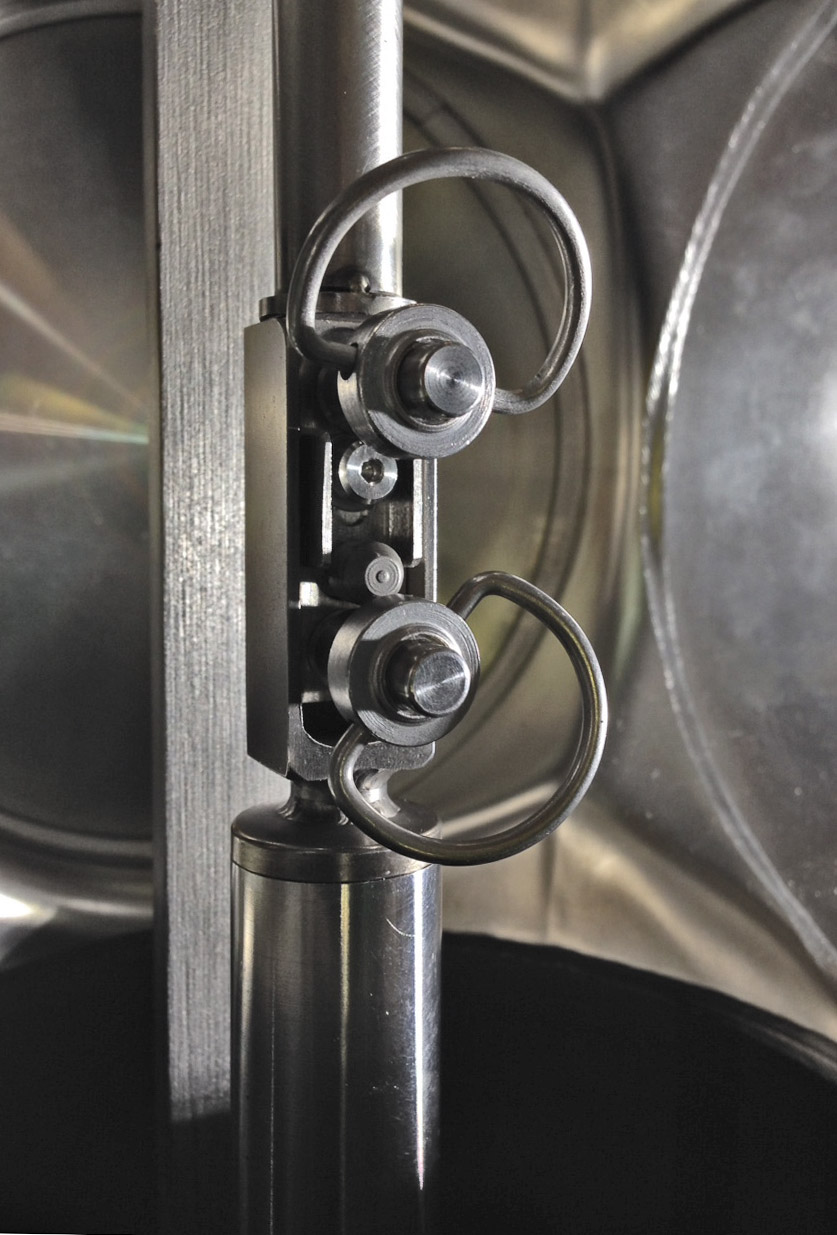
\includegraphics[width=3.2in]{Figs/sourceHolder_locking}
 \caption{Locking mechanism for the source holder. This photo shows two push pins that ensure that the sliding pin stays in place and the the source holder cannot under any circumstances get detached from the arm.  The only way to remove the push pins is to depress buttons on each of them by hand. }
 \label{fig:sourceHolder_locking}
\end{figure}

\begin{figure}[htbp]
 \centering
  \includegraphics[width=7in]{Figs/sourceAttachmentParts}
  \caption{Components of the source attachment mechanism. Central image shows how the pin that holds the source holder slides down and prevents the source from getting loose.  The slide pin is locked in place by two push pins shown in Fig. \ref{fig:sourceHolder_locking}}
  \label{fig:sourceAttachmentParts}
\end{figure}

\end{itemize}

 \subsubsection{Light Tightness}
 
   In order for CALIS III to be light tight, all view ports have light tight covers for when the organ pipe gate valve is open. When any view port or access port is opened, the gate valve must be closed, eliminating the possibility of leaking light into the veto. Additionally, all seals of CALIS III will be tested for leaks and confirmed to be helium leak tight. The gas tightness will be validated again after installation on the gate valve with gate valve closed. 
	
 \subsubsection{Vacuum evacuation and nitrogen purging}
 \paragraph{}
   One of the most important features of this system is making sure that the TMB and PC residue on the device are extracted from CALIS III prior to opening access ports to exchnage source or arms. This is  important for  safe working level of the people involved and for the detector.  This can be addressed through a system evacuation and nitrogen purge.  To accelerate the removal of the TMB in the scintillator fluid residue that is left after a deployment, CALIS III will undergo an evacuation with a vacuum pump. By lowering the pressure inside of CALIS below the vapor pressure of the TMB, it will cause the TMB to outgas and be removed through the vent line of the vacuum pump. An additional step to remove the TMB is to purge using N$_{2}$.  We will need to limit the potential flow rate of the nitrogen to ensure that an ODH (Oxygen Deficiency Hazard) condition is avoided in CRH.  Only once this is accomplished, will the view port be allowed to be opened and the source handled.     
  
The entire CALIS III  has been tested at FNAL  to hold pressure.  The system will be tested again after installation on the gate valve.
 

